\documentclass{standalone}
\usepackage{tikz}
\usetikzlibrary{patterns, positioning}


\begin{document}
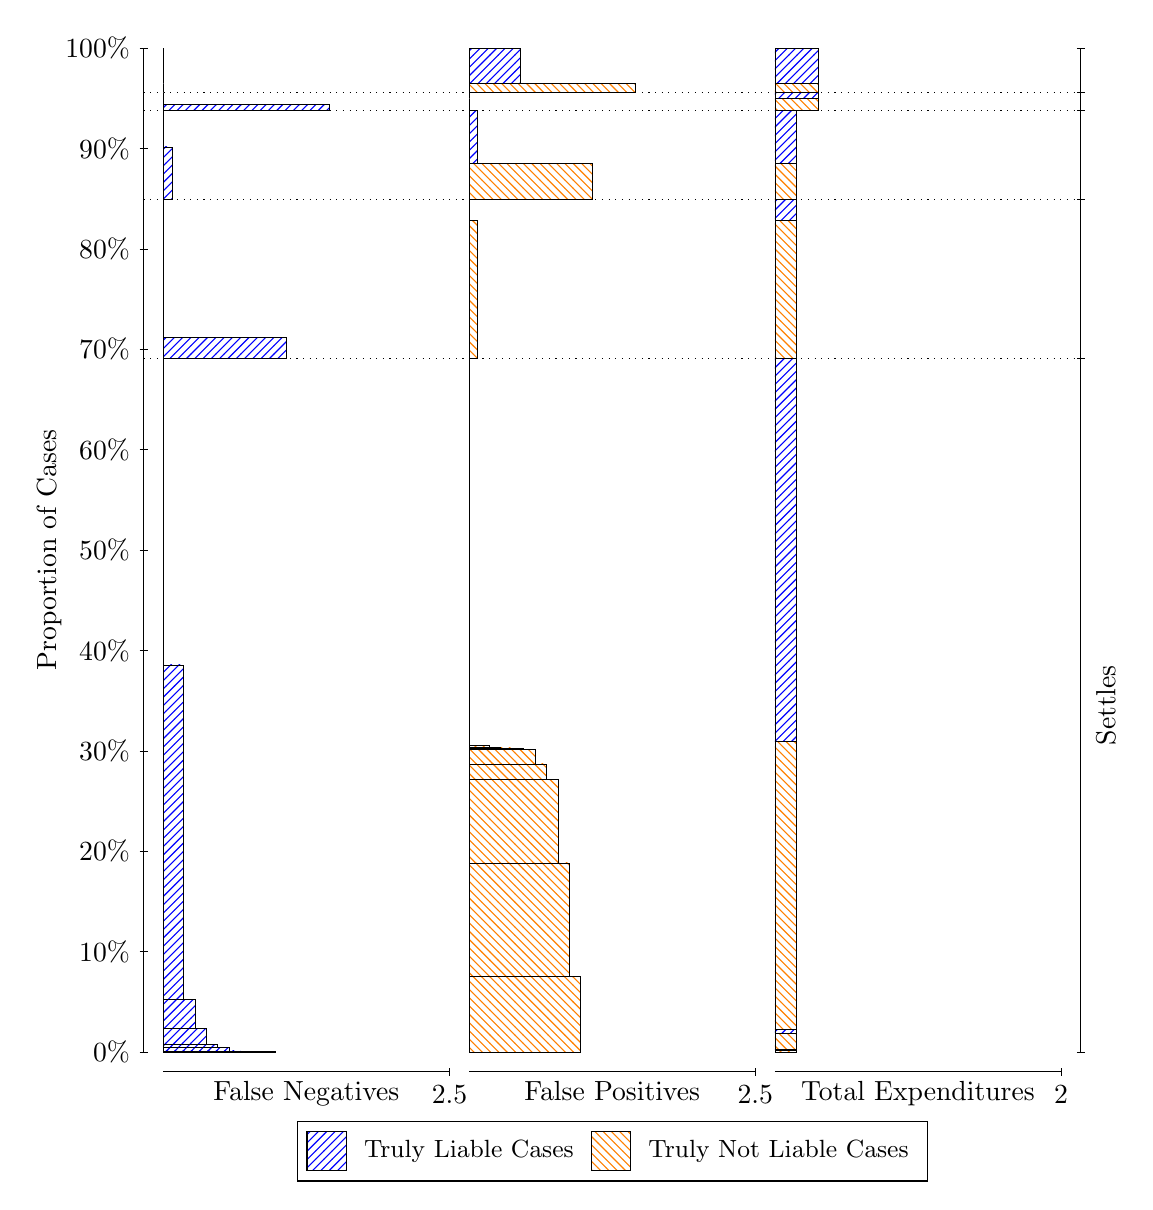
\begin{tikzpicture}
\draw[black, very thin] (1.5,1.75) -- (1.5,14.5);
\node[rotate=90, text=black, anchor=center] at (0.3, 8.125) {Proportion of Cases};
\draw[black, very thin] (1.45,1.75) -- (1.55,1.75);
\node[text=black, anchor=east] at (1.45, 1.75) {0\%};
\draw[black, very thin] (1.45,3.025) -- (1.55,3.025);
\node[text=black, anchor=east] at (1.45, 3.025) {10\%};
\draw[black, very thin] (1.45,4.3) -- (1.55,4.3);
\node[text=black, anchor=east] at (1.45, 4.3) {20\%};
\draw[black, very thin] (1.45,5.575) -- (1.55,5.575);
\node[text=black, anchor=east] at (1.45, 5.575) {30\%};
\draw[black, very thin] (1.45,6.85) -- (1.55,6.85);
\node[text=black, anchor=east] at (1.45, 6.85) {40\%};
\draw[black, very thin] (1.45,8.125) -- (1.55,8.125);
\node[text=black, anchor=east] at (1.45, 8.125) {50\%};
\draw[black, very thin] (1.45,9.4) -- (1.55,9.4);
\node[text=black, anchor=east] at (1.45, 9.4) {60\%};
\draw[black, very thin] (1.45,10.675) -- (1.55,10.675);
\node[text=black, anchor=east] at (1.45, 10.675) {70\%};
\draw[black, very thin] (1.45,11.95) -- (1.55,11.95);
\node[text=black, anchor=east] at (1.45, 11.95) {80\%};
\draw[black, very thin] (1.45,13.225) -- (1.55,13.225);
\node[text=black, anchor=east] at (1.45, 13.225) {90\%};
\draw[black, very thin] (1.45,14.5) -- (1.55,14.5);
\node[text=black, anchor=east] at (1.45, 14.5) {100\%};

\draw[black, very thin] (13.4,1.75) -- (13.4,14.5);
\draw[black, very thin] (13.35,1.75) -- (13.45,1.75);
\node[anchor=west] at (13.35, 1.75) {};
\draw[black, very thin] (13.35,10.556) -- (13.45,10.556);
\node[anchor=west] at (13.35, 10.556) {};
\draw[black, very thin] (13.35,12.577) -- (13.45,12.577);
\node[anchor=west] at (13.35, 12.577) {};
\draw[black, very thin] (13.35,13.705) -- (13.45,13.705);
\node[anchor=west] at (13.35, 13.705) {};
\draw[black, very thin] (13.35,13.938) -- (13.45,13.938);
\node[anchor=west] at (13.35, 13.938) {};
\draw[black, very thin] (13.35,14.5) -- (13.45,14.5);
\node[anchor=west] at (13.35, 14.5) {};

\draw[black, very thin, pattern color=blue, pattern=north east lines] (1.75,1.75) rectangle (3.167,1.7557);
\draw[black, very thin, pattern color=blue, pattern=north east lines] (1.75,1.7557) rectangle (3.0217,1.7566);
\draw[black, very thin, pattern color=blue, pattern=north east lines] (1.75,1.7566) rectangle (2.8763,1.7594);
\draw[black, very thin, pattern color=blue, pattern=north east lines] (1.75,1.7594) rectangle (2.731,1.7637);
\draw[black, very thin, pattern color=blue, pattern=north east lines] (1.75,1.7637) rectangle (2.5857,1.8045);
\draw[black, very thin, pattern color=blue, pattern=north east lines] (1.75,1.8045) rectangle (2.4403,1.8487);
\draw[black, very thin, pattern color=blue, pattern=north east lines] (1.75,1.8487) rectangle (2.295,2.0458);
\draw[black, very thin, pattern color=blue, pattern=north east lines] (1.75,2.0458) rectangle (2.1497,2.415);
\draw[black, very thin, pattern color=blue, pattern=north east lines] (1.75,2.415) rectangle (2.0043,6.6657);
\draw[black, very thin, pattern color=orange, pattern=north west lines] (1.75,6.6657) rectangle (1.75,10.556);
\draw[black, very thin, pattern color=blue, pattern=north east lines] (1.75,10.556) rectangle (3.3123,10.821);
\draw[black, very thin, pattern color=orange, pattern=north west lines] (1.75,10.821) rectangle (1.75,12.577);
\draw[black, very thin, pattern color=blue, pattern=north east lines] (1.75,12.577) rectangle (1.859,13.244);
\draw[black, very thin, pattern color=orange, pattern=north west lines] (1.75,13.244) rectangle (1.75,13.705);
\draw[black, very thin, pattern color=blue, pattern=north east lines] (1.75,13.705) rectangle (3.8573,13.784);
\draw[black, very thin, pattern color=orange, pattern=north west lines] (1.75,13.784) rectangle (1.75,13.938);
\draw[black, very thin, pattern color=orange, pattern=north west lines] (1.75,13.938) rectangle (1.75,14.051);
\draw[black, very thin, pattern color=blue, pattern=north east lines] (1.75,14.051) rectangle (1.75,14.5);
\draw[black, very thin, pattern color=orange, pattern=north west lines] (5.6333,1.75) rectangle (7.0503,2.7115);
\draw[black, very thin, pattern color=orange, pattern=north west lines] (5.6333,2.7115) rectangle (6.905,4.152);
\draw[black, very thin, pattern color=orange, pattern=north west lines] (5.6333,4.152) rectangle (6.7597,5.2155);
\draw[black, very thin, pattern color=orange, pattern=north west lines] (5.6333,5.2155) rectangle (6.6143,5.4088);
\draw[black, very thin, pattern color=orange, pattern=north west lines] (5.6333,5.4088) rectangle (6.469,5.5892);
\draw[black, very thin, pattern color=orange, pattern=north west lines] (5.6333,5.5892) rectangle (6.3237,5.5932);
\draw[black, very thin, pattern color=orange, pattern=north west lines] (5.6333,5.5932) rectangle (6.3237,5.6015);
\draw[black, very thin, pattern color=orange, pattern=north west lines] (5.6333,5.6015) rectangle (6.1783,5.6105);
\draw[black, very thin, pattern color=orange, pattern=north west lines] (5.6333,5.6105) rectangle (6.033,5.6146);
\draw[black, very thin, pattern color=orange, pattern=north west lines] (5.6333,5.6146) rectangle (5.8877,5.6408);
\draw[black, very thin, pattern color=blue, pattern=north east lines] (5.6333,5.6408) rectangle (5.6333,10.556);
\draw[black, very thin, pattern color=orange, pattern=north west lines] (5.6333,10.556) rectangle (5.7423,12.313);
\draw[black, very thin, pattern color=blue, pattern=north east lines] (5.6333,12.313) rectangle (5.6333,12.577);
\draw[black, very thin, pattern color=orange, pattern=north west lines] (5.6333,12.577) rectangle (7.1957,13.039);
\draw[black, very thin, pattern color=blue, pattern=north east lines] (5.6333,13.039) rectangle (5.7423,13.705);
\draw[black, very thin, pattern color=orange, pattern=north west lines] (5.6333,13.705) rectangle (5.6333,13.859);
\draw[black, very thin, pattern color=blue, pattern=north east lines] (5.6333,13.859) rectangle (5.6333,13.938);
\draw[black, very thin, pattern color=orange, pattern=north west lines] (5.6333,13.938) rectangle (7.7407,14.051);
\draw[black, very thin, pattern color=blue, pattern=north east lines] (5.6333,14.051) rectangle (6.2873,14.5);
\draw[black, very thin, pattern color=orange, pattern=north west lines] (9.5167,1.75) rectangle (9.7892,1.7754);
\draw[black, very thin, pattern color=blue, pattern=north east lines] (9.5167,1.7754) rectangle (9.7892,1.7833);
\draw[black, very thin, pattern color=orange, pattern=north west lines] (9.5167,1.7833) rectangle (9.7892,1.99);
\draw[black, very thin, pattern color=blue, pattern=north east lines] (9.5167,1.99) rectangle (9.7892,2.0365);
\draw[black, very thin, pattern color=orange, pattern=north west lines] (9.5167,2.0365) rectangle (9.7892,5.6953);
\draw[black, very thin, pattern color=blue, pattern=north east lines] (9.5167,5.6953) rectangle (9.7892,10.556);
\draw[black, very thin, pattern color=orange, pattern=north west lines] (9.5167,10.556) rectangle (9.7892,12.313);
\draw[black, very thin, pattern color=blue, pattern=north east lines] (9.5167,12.313) rectangle (9.7892,12.577);
\draw[black, very thin, pattern color=orange, pattern=north west lines] (9.5167,12.577) rectangle (9.7892,13.039);
\draw[black, very thin, pattern color=blue, pattern=north east lines] (9.5167,13.039) rectangle (9.7892,13.705);
\draw[black, very thin, pattern color=orange, pattern=north west lines] (9.5167,13.705) rectangle (10.062,13.859);
\draw[black, very thin, pattern color=blue, pattern=north east lines] (9.5167,13.859) rectangle (10.062,13.938);
\draw[black, very thin, pattern color=orange, pattern=north west lines] (9.5167,13.938) rectangle (10.062,14.051);
\draw[black, very thin, pattern color=blue, pattern=north east lines] (9.5167,14.051) rectangle (10.062,14.5);
\draw[black, dotted] (1.5,10.556) -- (13.4,10.556);
\draw[black, dotted] (1.5,12.577) -- (13.4,12.577);
\draw[black, dotted] (1.5,13.705) -- (13.4,13.705);
\draw[black, dotted] (1.5,13.938) -- (13.4,13.938);
\draw[black, very thin] (1.75,1.5) -- (5.3833,1.5);
\node[text=black, anchor=north] at (3.5667, 1.5) {False Negatives};
\draw[black, very thin] (5.3833,1.45) -- (5.3833,1.55);
\node[text=black, anchor=north] at (5.3833, 1.45) {2.5};

\draw[black, very thin] (5.6333,1.5) -- (9.2667,1.5);
\node[text=black, anchor=north] at (7.45, 1.5) {False Positives};
\draw[black, very thin] (9.2667,1.45) -- (9.2667,1.55);
\node[text=black, anchor=north] at (9.2667, 1.45) {2.5};

\draw[black, very thin] (9.5167,1.5) -- (13.15,1.5);
\node[text=black, anchor=north] at (11.333, 1.5) {Total Expenditures};
\draw[black, very thin] (13.15,1.45) -- (13.15,1.55);
\node[text=black, anchor=north] at (13.15, 1.45) {2};

\node[text=black, centered, rotate=90] at (13.72, 6.1532) {Settles};





\draw (7.449999999999999,1.5) node[draw=none] (baseCoordinate) {};
\begin{scope}[align=center]
        \matrix[scale=0.5, draw=black, below=0.5cm of baseCoordinate, nodes={draw}, column sep=0.1cm]{
            \node[rectangle, draw, minimum width=0.5cm, minimum height=0.5cm, pattern color=blue, pattern=north east lines] {}; &
            \node[draw=none, font=\small, text=black] (B) {Truly Liable Cases}; &
            \node[rectangle, draw, minimum width=0.5cm, minimum height=0.5cm, pattern color=orange, pattern=north west lines] {}; &
            \node[draw=none, font=\small, text=black] (B) {Truly Not Liable Cases}; \\
            };
\end{scope}

\end{tikzpicture}
\end{document}